\chapter{Experimentación}
\label{cap:experimentacion}
Este capítulo muestra algunas de las pruebas realizadas y los resultados obtenidos.
Se comparan diferentes estrategias en los dos juegos desarrollados.
Para ello se han realizado varias simulaciones y análisis de estados con las estrategias.

La siguiente sección se centra en las pruebas realizadas a los evaluadores heurísticos de cada juego, incluyendo algunas series de entrenamientos para los evaluadores entrenables.

\section{Comparativa de evaluadores heurísticos}  
\label{sec:comparativa_evaluadores_heuristicos}
Primero se han comparado los evaluadores heurísticos de cada uno de los juegos de forma independiente.

\subsection{Evaluadores del Conecta-4}
\label{ssec:comparativa_evaluadores_conecta4}
Para comparar los evaluadores heurísticos del Conecta-4 se han jugado 100 partidas entre un jugador evaluador (\texttt{JugadorEvaluar}) y un jugador aleatorio para cada prueba.
Recordemos que un \texttt{JugadorEvaluar} considera todos los movimientos inmediatos, los evalúa heurísticamente y escoge el mejor.

Las pruebas se han realizado en un tablero de dimensiones 6x7 con una longitud ganadora de cuatro fichas.
Los evaluadores heurísticos usados son la matriz de posibilidades (número de posibilidades de conectar cuatro fichas de \textit{MAX} menos el número de posibilidades de conectar cuatro fichas que tiene \textit{MIN}), la tabla de valor y la red neuronal.
La tabla de valor y la red neuronal se han entrenado con 2.000 partidas frente a un jugador aleatorio, con una tasa de aprendizaje de 0.1 y una tasa de exploración de 0.1.
La red neuronal cuenta con una única neurona en la capa intermedia.

Las tablas~\ref{tab:comparativa_heuristicos_conecta4_jug1} y \ref{tab:comparativa_heuristicos_conecta4_jug2} presentan los resultados de las pruebas realizadas con el \texttt{JugadorEvaluar} jugando como primer jugador y como segundo jugador respectivamente.
Las figuras~\ref{fig:comparativa_heuristicos_conecta4_jug1} y \ref{fig:comparativa_heuristicos_conecta4_jug2} muestran de forma gráfica estos resultados. 

% HEURISTICOS CONECTA-4
\begin{table}[!h]
\centering
\caption[Comparativa de los evaluadores heurísticos del Conecta-4 (I)]{Comparativa de los evaluadores heurísticos del Conecta-4 para el primer jugador.}
\label{tab:comparativa_heuristicos_conecta4_jug1}
\begin{tabular}{lccc}
\hline
\textbf{Jugador 1:} & \textbf{Ev. Heur. (Matriz de posibilidades)} & \textbf{Tabla de valor} & \textbf{Red neuronal} \\
%\hline
\textbf{Gana} & 98\% & 84\% & 88\% \\
\textbf{Empata} & 0\% & 0\% & 0\% \\
\textbf{Pierde} & 2\% & 16\% & 12\% \\
\hline
\end{tabular}
\end{table} 

\begin{figure}[!h]
	\centering
	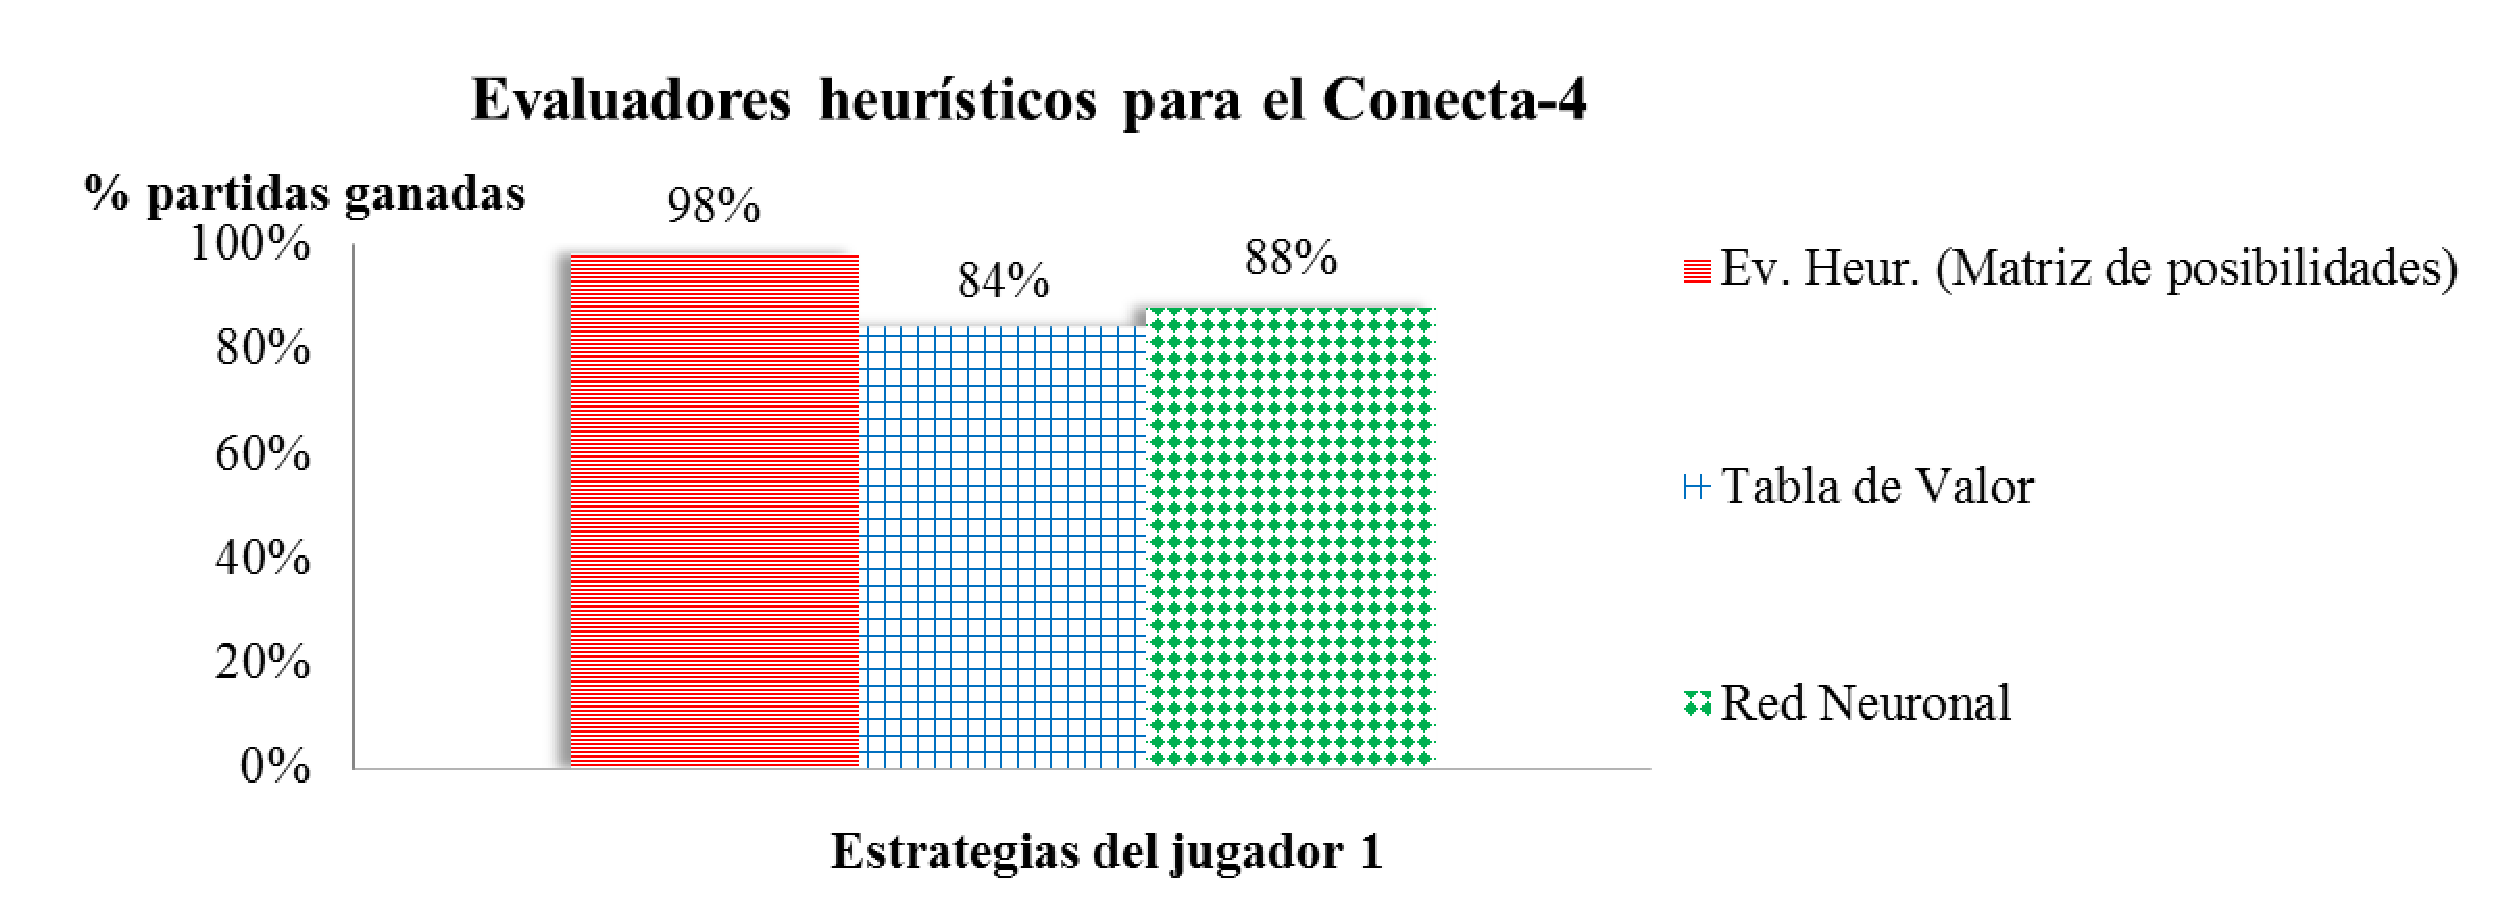
\includegraphics[scale=0.3]{contenido/cap7/imagenes/heuristicosConecta4jug1.eps}
	\caption[Comparativa de los evaluadores heurísticos del Conecta-4 (I)]{Gráfica comparativa de los evaluadores heurísticos del Conecta-4 para el primer jugador.}
	\label{fig:comparativa_heuristicos_conecta4_jug1}
\end{figure}

\begin{table}[!h]
\centering
\caption[Comparativa de los evaluadores heurísticos del Conecta-4 (II)]{Comparativa de los evaluadores heurísticos del Conecta-4 para el segundo jugador.}
\label{tab:comparativa_heuristicos_conecta4_jug2}
\begin{tabular}{lccc}
\hline
\textbf{Jugador 2:} & \textbf{Ev. Heur. (Matriz de posibilidades)} & \textbf{Tabla de valor} & \textbf{Red neuronal} \\
%\hline
\textbf{Gana} & 94\% & 78\% & 81\% \\
\textbf{Empata} & 0\% & 0\% & 1\% \\
\textbf{Pierde} & 6\% & 22\% & 18\% \\
\hline
\end{tabular}
\end{table} 

\begin{figure}[!h]
	\centering
	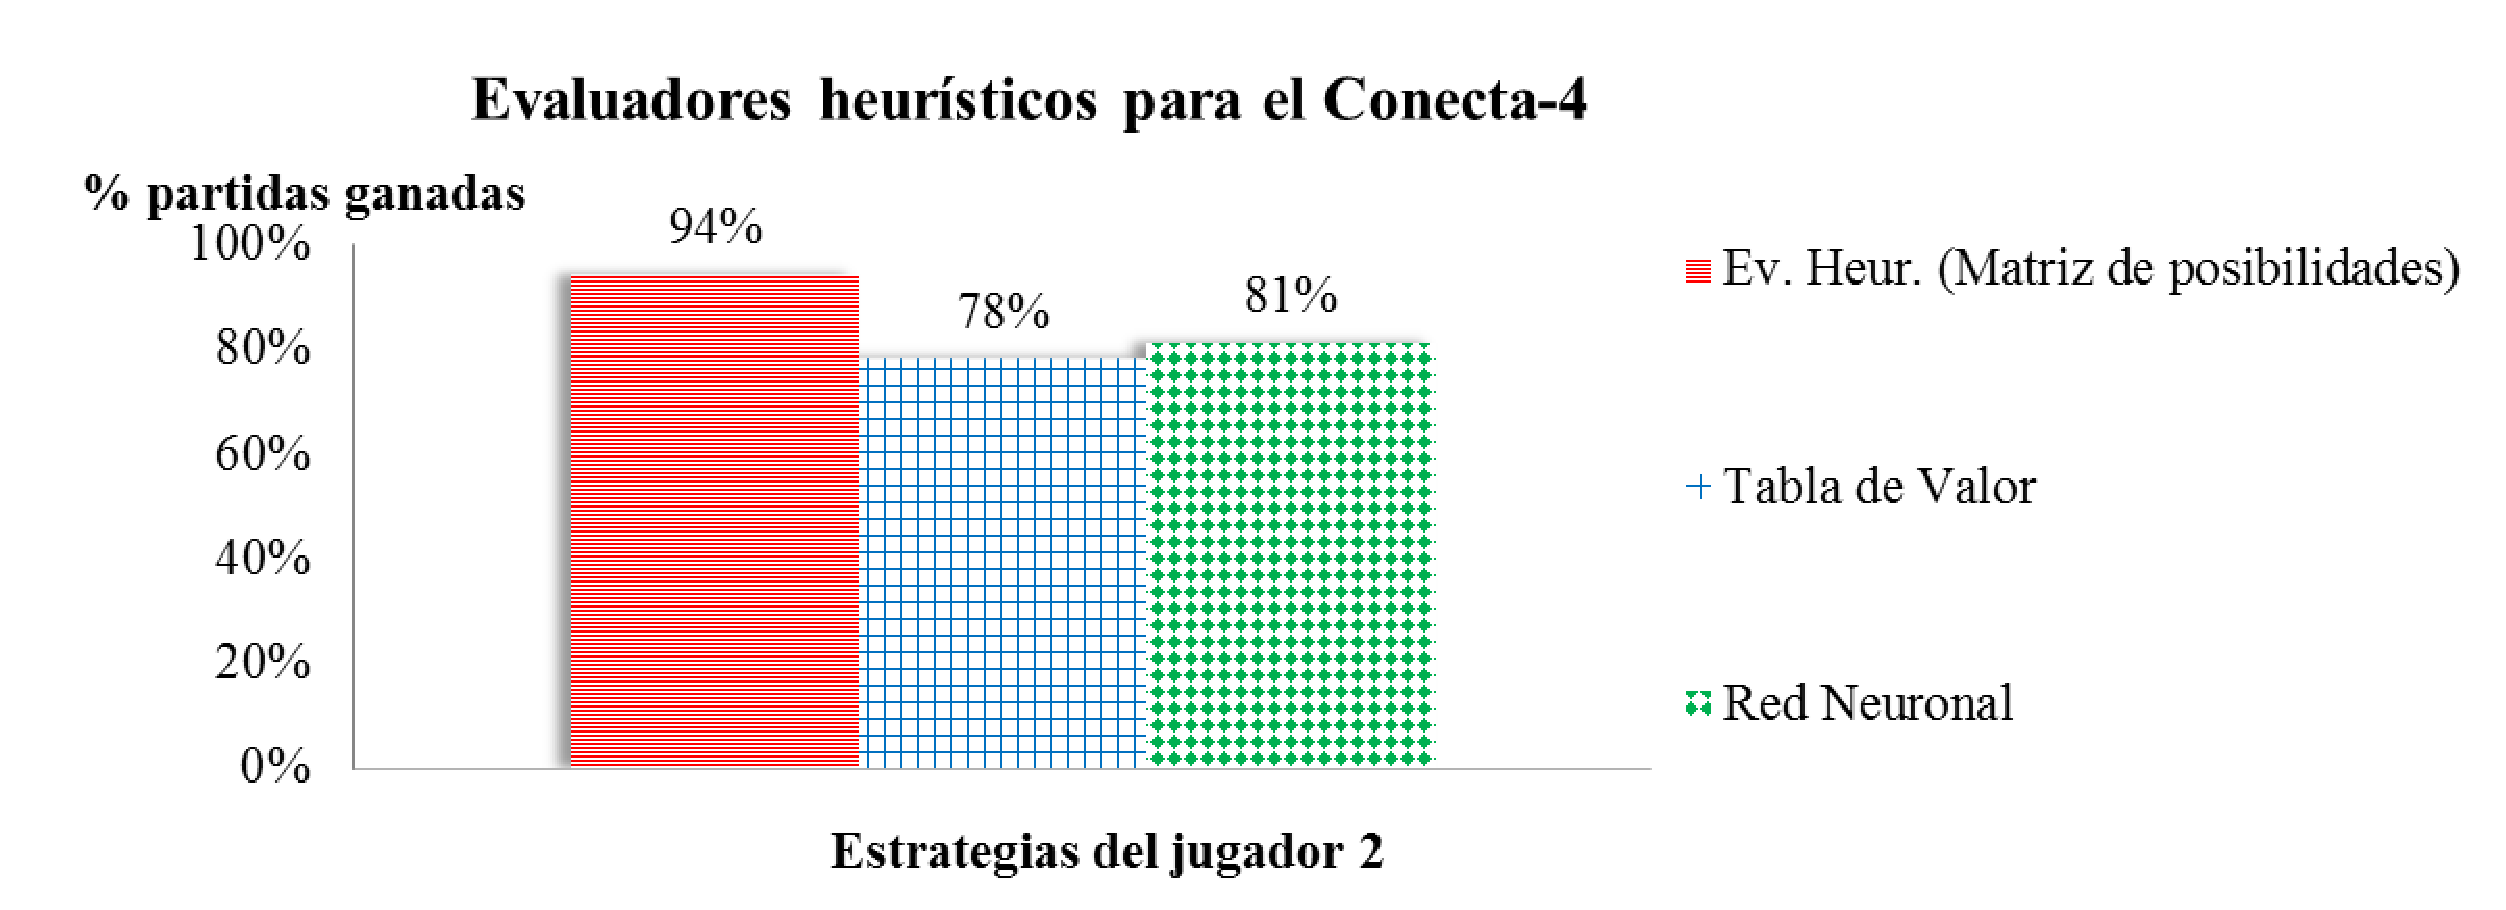
\includegraphics[scale=0.3]{contenido/cap7/imagenes/heuristicosConecta4jug2.eps}
	\caption[Comparativa de los evaluadores heurísticos del Conecta-4 (II)]{Gráfica comparativa de los evaluadores heurísticos del Conecta-4 para el segundo jugador.}
	\label{fig:comparativa_heuristicos_conecta4_jug2}
\end{figure} 
 
Se observa que un evaluador que utilice información de la situación actual del juego para realizar la evaluación ofrece mejores resultados que un evaluador que no tenga en cuenta esa información; aunque en este caso, con un número mayor de partidas de entrenamiento se pueden conseguir los mismos resultados.

\subsection{Evaluadores del Go}
\label{ssec:comparativa_evaluadores_go}
Para el juego del Go también también se han jugado 100 partidas entre un \texttt{JugadorEvaluar} y un jugador aleatorio para cada prueba.
Las pruebas se han realizado en un tablero de dimensiones 9x9, con las reglas de puntuación japonesas y sin puntos de ventaja para el segundo jugador.

Las tablas~\ref{tab:comparativa_heuristicos_go_jug1} y \ref{tab:comparativa_heuristicos_go_jug2} presentan los resultados de las pruebas para el juego del Go y las figuras~\ref{fig:comparativa_heuristicos_go_jug1} y \ref{fig:comparativa_heuristicos_go_jug2} muestran de forma gráfica los resultados. 
Los evaluadores heurísticos usados han sido un evaluador basado en el número de territorios (Territorios), uno basado en los puntos según las reglas chinas (P. CH), otro basado en los puntos según las reglas japonesas (P. JP), la tabla de valor y la red neuronal.
La tabla de valor y la red neuronal se han entrenado con 2.000 partidas frente a un jugador aleatorio, con los mismos parámetros de entrenamiento que en el experimento anterior.
La red neuronal cuenta con nueve neuronas en la capa intermedia.

% HEURISTICOS GO
\begin{table}[!h]
\centering
\caption[Comparativa de los evaluadores heurísticos del Go (I)]{Comparativa de los evaluadores heurísticos del Go para el primer jugador.}
\label{tab:comparativa_heuristicos_go_jug1}
\begin{tabular}{lccccc}
\hline
\textbf{Jugador 1:} & \textbf{Territorios} & \textbf{P. CH} & \textbf{P. JP} & \textbf{Tabla de valor} & \textbf{Red neuronal} \\
%\hline
\textbf{Gana} & 94\% & 100\% & 97\% & 72\% & 99\% \\
\textbf{Empata} & 0\% & 0\% & 0\% & 0\% & 0\% \\
\textbf{Pierde} & 6\% & 0\% & 3\% & 24\% & 1\% \\
\hline
\end{tabular}
\end{table} 

\begin{figure}[!h]
	\centering
	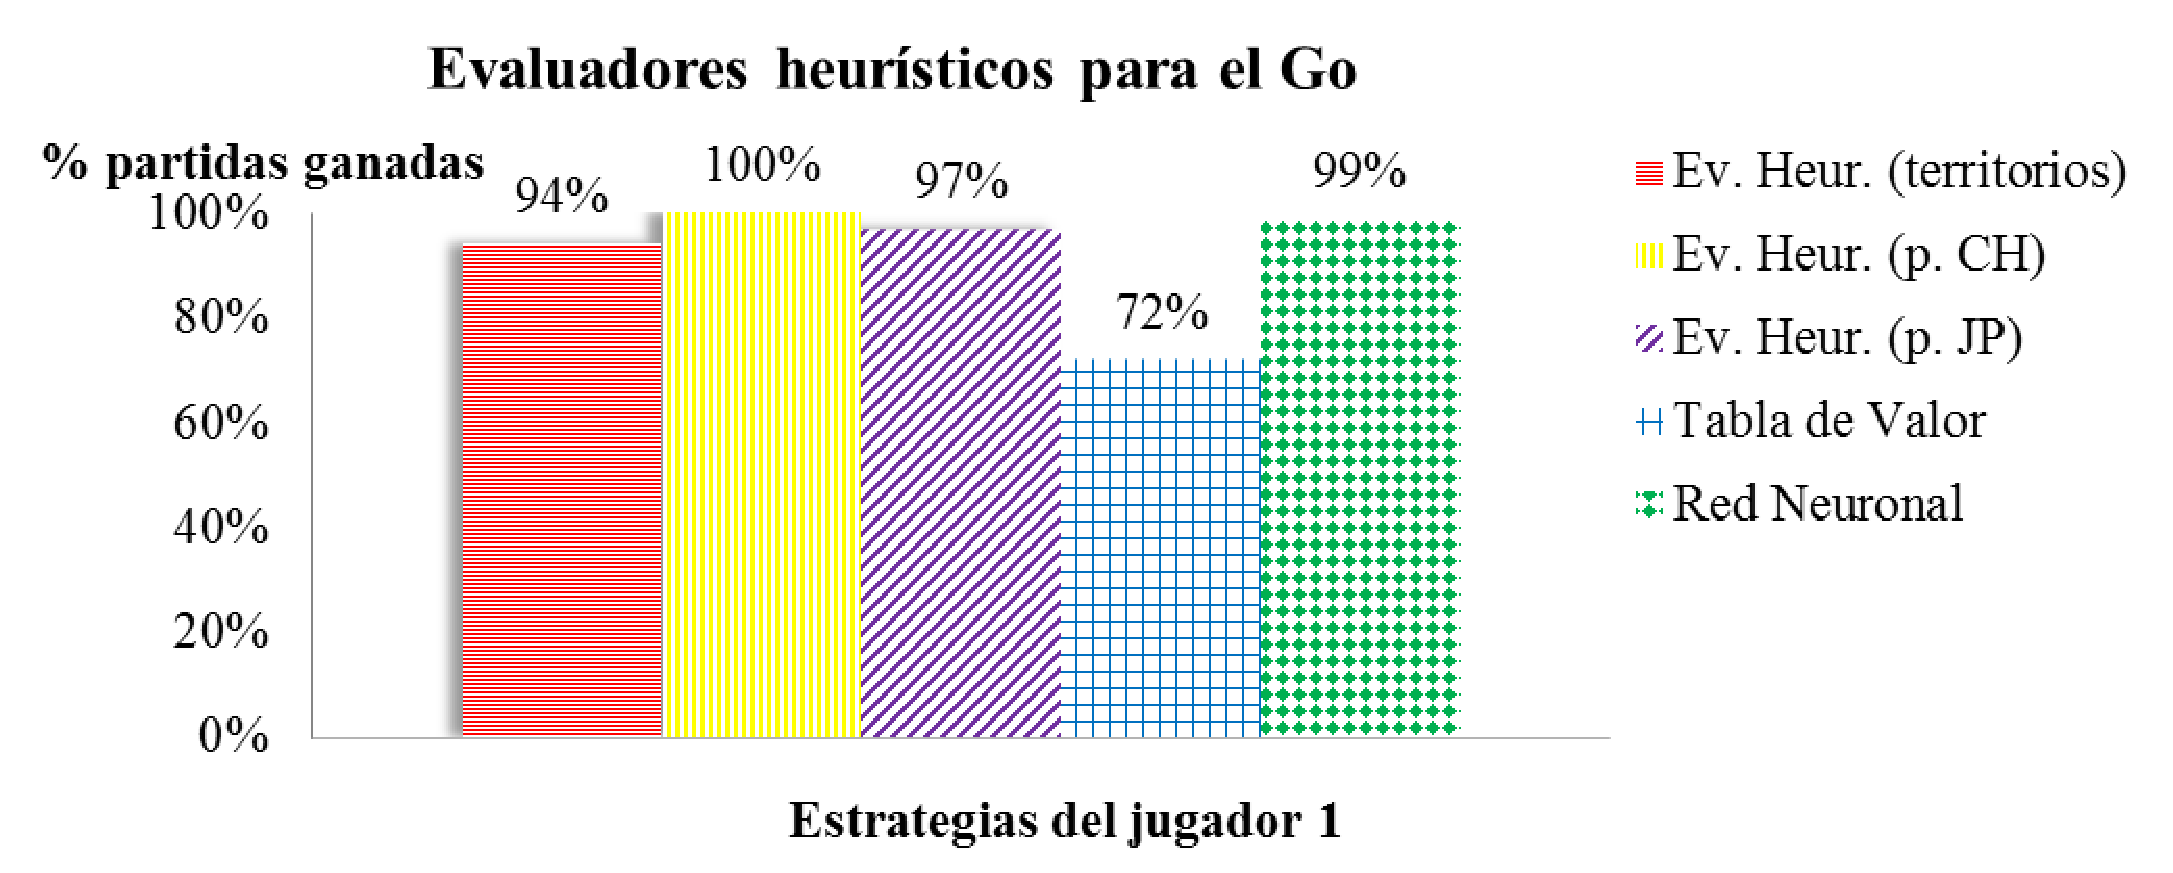
\includegraphics[scale=0.3]{contenido/cap7/imagenes/heuristicosGojug1.eps}
	\caption[Comparativa de los evaluadores heurísticos del Go (I)]{Gráfica comparativa de los evaluadores heurísticos del Go para el primer jugador.}
	\label{fig:comparativa_heuristicos_go_jug1}
\end{figure}

\begin{table}[b]
\centering
\caption[Comparativa de los evaluadores heurísticos del Go (II)]{Comparativa de los evaluadores heurísticos del Go para el segundo jugador.}
\label{tab:comparativa_heuristicos_go_jug2}
\begin{tabular}{lccccc}
\hline
\textbf{Jugador 2:} & \textbf{Territorios} & \textbf{P. CH} & \textbf{P. JP} & \textbf{Tabla de valor} & \textbf{Red neuronal} \\
%\hline
\textbf{Gana} & 93\% & 99\% & 95\% & 67\% & 65\% \\
\textbf{Empata} & 0\% & 0\% & 0\% & 1\% & 2\% \\
\textbf{Pierde} & 7\% & 1\% & 5\% & 32\% & 33\% \\
\hline
\end{tabular}
\end{table} 

\begin{figure}[!h]
	\centering
	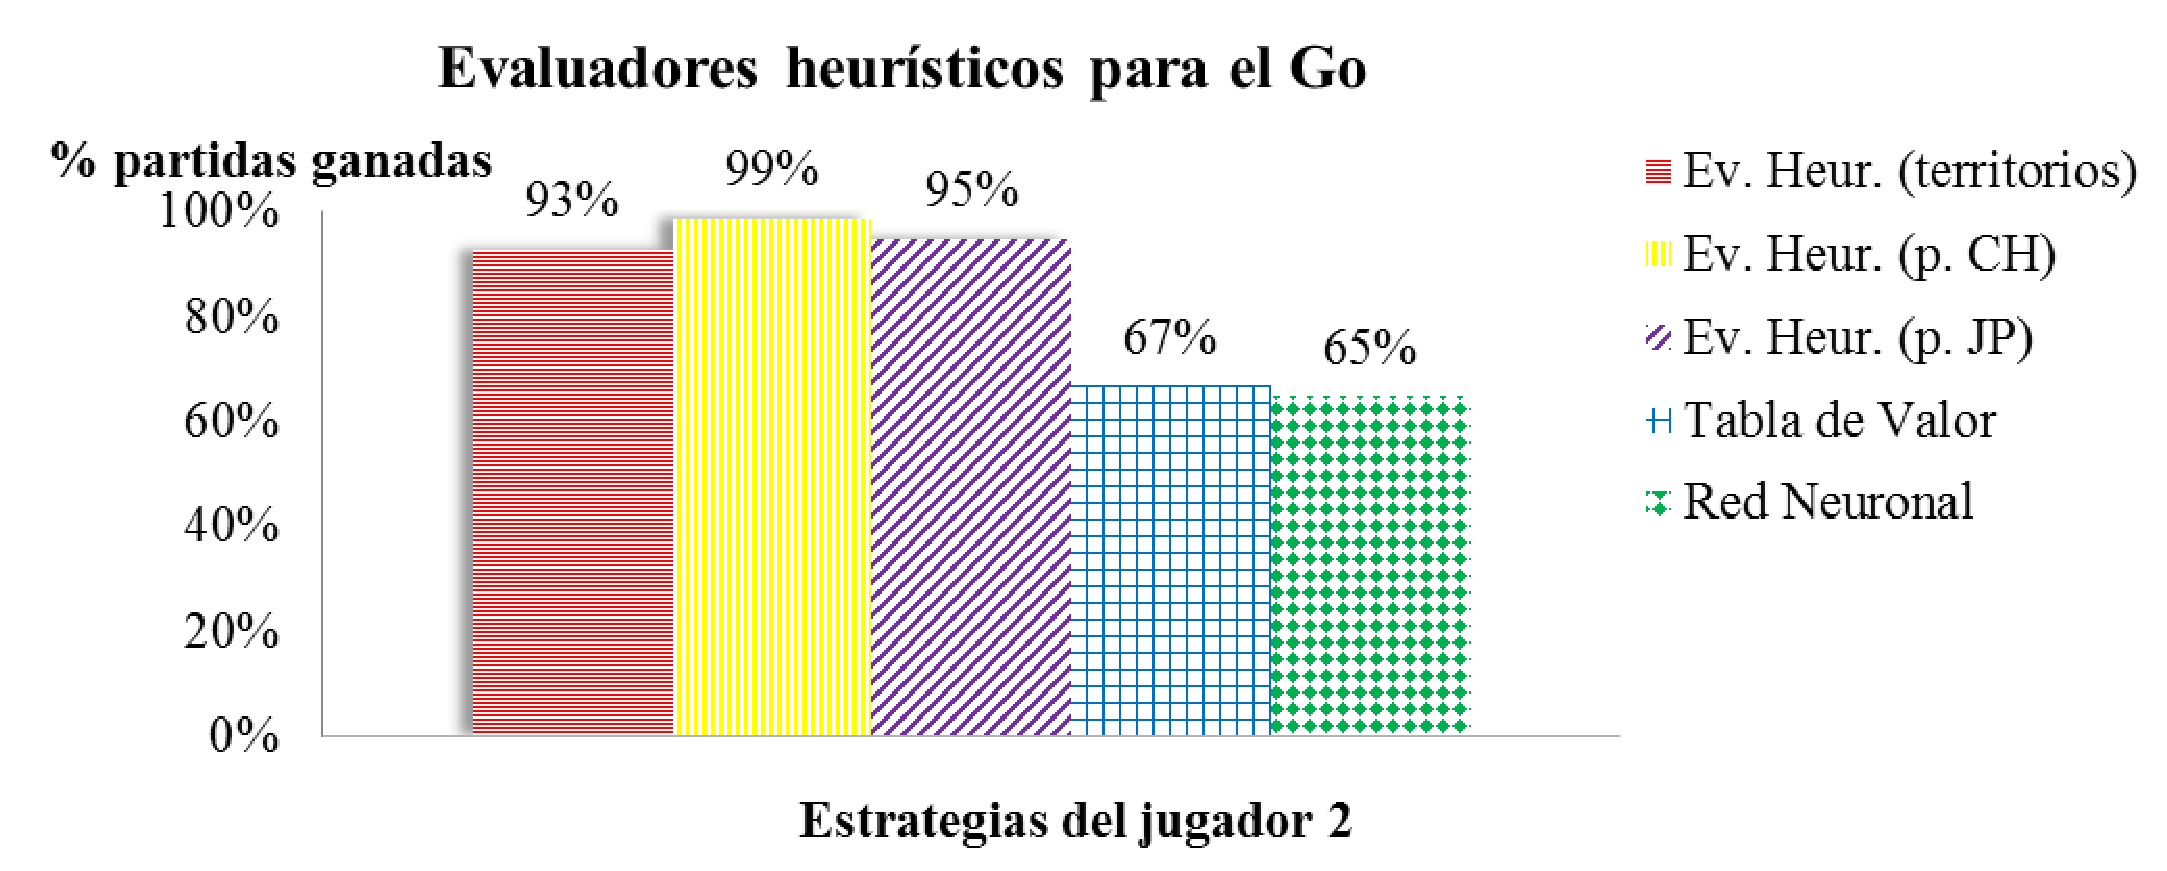
\includegraphics[scale=0.3]{contenido/cap7/imagenes/heuristicosGojug2.eps}
	\caption[Comparativa de los evaluadores heurísticos del Go (II)]{Gráfica comparativa de los evaluadores heurísticos del Go para el segundo jugador.}
	\label{fig:comparativa_heuristicos_go_jug2}
\end{figure} 

En el caso del Go la diferencia entre los evaluadores que usan información del dominio y los que no es más evidente, sobre todo para el segundo jugador; esto se debe a que el tamaño del espacio de estados del Go es mayor que el del Conecta-4, lo que además hace que una estrategia aleatoria sea muy fácil de vencer.
Los evaluadores entrenables también necesitan más partidas de entrenamiento para conseguir los mismos resultados que el resto de evaluadores.

\subsection{Entrenamientos}
\label{ssec:comparativa_entrenamientos}
En esta sección se estudian varias secuencias de entrenamiento en el juego del Go.
Se ha considerado un tablero 9x9 con las reglas de puntuación japonesas y sin ninguna ventaja para el segundo jugador.

Se entrenan cuatro jugadores diferentes con red neuronal (\texttt{JugadorEvaluar}): uno como primer jugador frente a una estrategia aleatoria (J1), otro como segundo jugador frente a una estrategia aleatoria (J2) y los otros dos jugadores se entrenan simultáneamente uno frente al otro (J3 y J4).
En todos los casos la red neuronal dispone de nueve neuronas en la capa intermedia y los pesos iniciales son aleatorios, la tasa de aprendizaje para ajustar la velocidad a la que aprende la red tiene un valor de 0.1 y el momento de entrenamiento que indica la influencia que tiene la iteración anterior sobre la actual es de 0.8.

Las tablas~\ref{tab:secuencia1}, \ref{tab:secuencia2} y \ref{tab:secuencia2} muestran cómo evoluciona el aprendizaje de la red neuronal para cada uno de los casos.
Las tres secuencias de entrenamiento constan de 2.000 partidas, mostrándose cada 100 los resultados de 100 partidas sin aprendizaje.
En todos los casos se toman las últimas redes, es decir, las obtenidas después de los entrenamiento completos de 2.000 partidas, independientemente de los resultados obtenidos durante el proceso.
Esto puede dar lugar a un sobreaprendizaje, como se observa en la secuencia 3.

Las figuras~\ref{fig:secuencia1}, \ref{fig:secuencia2} y \ref{fig:secuencia3} muestran de forma gráfica la evolución del aprendizaje para cada secuencia de entrenamiento.

\begin{table}[t]
	\centering
	% Primera imagen
	\begin{minipage}[t]{0.4\linewidth}
		\centering
		\caption[Secuencia de entrenamiento 1]{Secuencia 1.}
		\label{tab:secuencia1}
				{\footnotesize
				\begin{tabular}{rrrr}
\hline
\textbf{Nº partidas} & \textbf{J1} & \textbf{Empate} & \textbf{Aleatorio} \\
%\hline
0	& 42\% &	4\%	& 54\% \\
100	& 41\% &	3\%	& 56\% \\
200	& 24\% &	8\%	& 68\% \\
300	& 37\% &	3\%	& 60\% \\
400	& 21\% &	5\%	& 74\% \\
500	& 25\% &	4\%	& 71\% \\
600	& 63\% &	3\%	& 34\% \\
700	& 67\% &	1\%	& 32\% \\
800	& 43\% &	3\%	& 54\% \\
900	& 61\% &	0\%	& 39\% \\
1000 &	57\% &	0\%	& 43\% \\
1100 &	87\% &	0\%	& 13\% \\
1200 &	87\% &	0\%	& 13\% \\
1300 &	73\% &	0\%	& 27\% \\
1400 &	94\% &	0\%	& 6\% \\
1500 &	99\% &	0\%	& 1\% \\
1600 &	98\% &	0\%	& 2\% \\
1700 &	97\% &	0\%	& 3\% \\
1800 &	98\% &	0\%	& 2\% \\
1900 &	98\% &	0\%	& 2\% \\
2000 &	96\% &	0\%	& 4\% \\
\hline
\end{tabular}
}
	\end{minipage}
	\hspace{1cm}
	% Segunda imagen
	\begin{minipage}[t]{0.4\linewidth}
		\centering
		\caption[Secuencia de entrenamiento 2]{Secuencia 2.}
		\label{tab:secuencia2}
			{\footnotesize
				\begin{tabular}{rrrr}
\hline
\textbf{Nº partidas} & \textbf{Aleatorio} & \textbf{Empate} & \textbf{J2} \\
%\hline
0	& 50\% &	0\% &	48\% \\
100	& 35\% &	0\% &	61\% \\
200	& 43\% &	0\% &	51\% \\
300	& 53\% &	0\% &	45\% \\
400	& 37\% &	0\% &	61\% \\
500	& 35\% &	0\% &	65\% \\
600	& 49\% &	0\% &	51\% \\
700	& 51\% &	0\% &	47\% \\
800	& 8\% &	0\%	 &92\% \\
900	& 6\% &	0\%	 &94\% \\
1000 &	14\% &	0\%	 & 85\% \\
1100 &	17\% &	0\%	 & 82\% \\
1200 &	33\% &	0\%	 & 65\% \\
1300 &	15\% &	0\% &	85\% \\
1400 &	11\% &	0\% &	89\% \\
1500 &	15\% &	0\% &	85\% \\
1600 &	12\% &	0\% &	88\% \\
1700 &	18\% &	0\% &	82\% \\
1800 &	16\% &	0\% &	84\% \\
1900 &	7\%	&   0\%	 & 93\% \\
2000 &	33\% &	0\% &	67\% \\
\hline
\end{tabular}
}
	\end{minipage}
\end{table}

\begin{table}[t]
\caption[Secuencia de entrenamiento 3]{Secuencia 3.}
\label{tab:secuencia3}
\centering
{\footnotesize
\begin{tabular}{rrrr}
\hline
\textbf{Nº partidas} & \textbf{Aleatorio} & \textbf{Empate} & \textbf{J2} \\
%\hline
0	& 0\% &	0\% &	100\% \\
100	&0\% &	0\% &	100\% \\
200	&0\% &	0\% &	100\% \\
300	&100\% &	0\% &	0\% \\
400	&100\% &	0\% &	0\% \\
500	&100\% &	0\% &	0\% \\
600	&100\% &	0\% &	0\% \\
700	&100\% &	0\% &	0\% \\
800	&0\% &	0\% &	100\% \\
900	&100\% &	0\% &	0\% \\
1000 &	0\% &	0\% &	100\% \\
1100 &	100\% &	0\% &	0\% \\
1200 &	0\% &	0\% &	100\% \\
1300 &	0\% &	100\% &	0\% \\
1400 &	0\% &	100\% &	0\% \\
1500 &	0\% &	100\% &	0\% \\
1600 &	0\% &	100\% &	0\% \\
1700 &	100\% &	0\% &	0\% \\
1800 &	0\% &	100\% &	0\% \\
1900 &	100\% &	0\% &	0\% \\
2000 &	100\% &	0\% &	0\% \\
\hline
\end{tabular}
}
\end{table} 

En el aprendizaje pueden presentarse oscilaciones, por lo que puede ser necesario cierto grado de experimentación antes de obtener una red correctamente entrenada.

Los valores de la secuencia número 3 pueden parecer extraños, esto se debe a que la red neuronal siempre devuelve el mismo movimiento para un estado dado y por lo tanto siempre se juegan las mismas partidas entre las dos redes neuronales; sin embargo, es más provechoso entrenar a dos jugadores simultáneamente (cada uno aprendiendo de su juego con el otro) que usando un jugador aleatorio.
A medida que se aumenta el tamaño del tablero de juego, el jugador aleatorio es menos eficaz para entrenar a los jugadores.

\begin{figure}[t]
	\centering
	% Primera imagen
	\begin{minipage}[t]{0.4\linewidth}
		\centering
		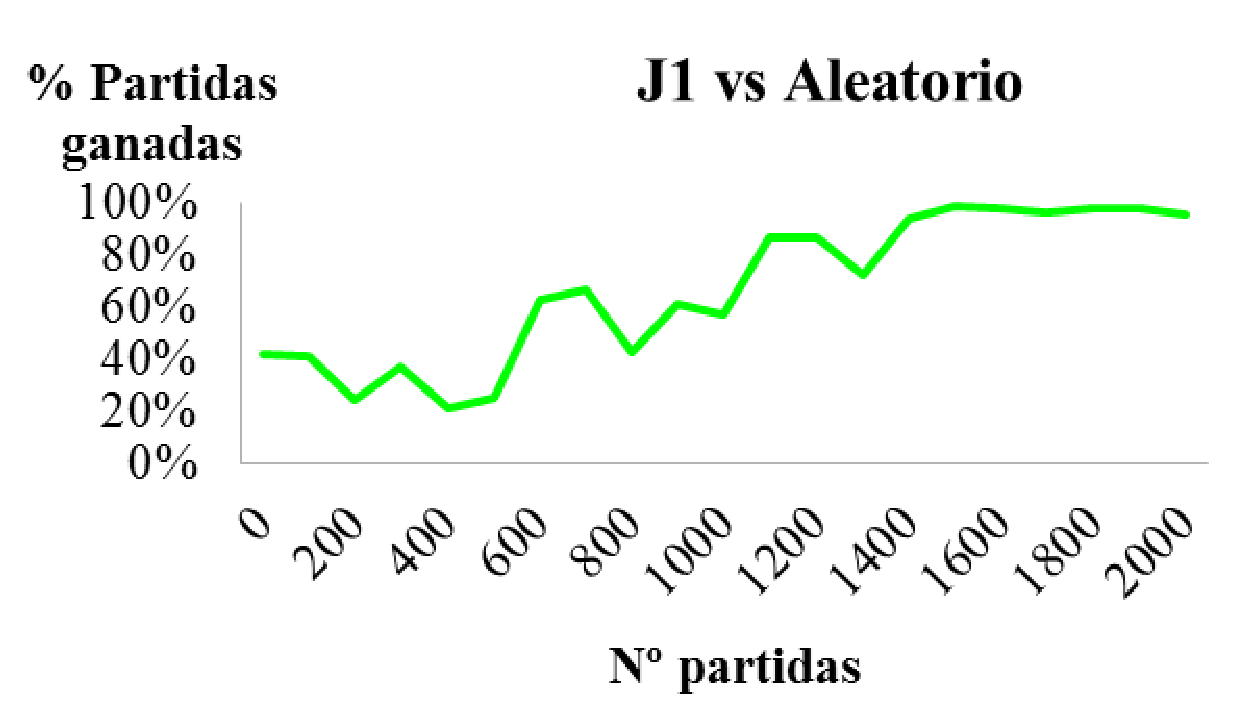
\includegraphics[scale=0.3]{contenido/cap7/imagenes/entrenamientoSecuencia1.eps}
		\caption[Secuencia de entrenamiento 1]{Secuencia 1.}
		\label{fig:secuencia1}
	\end{minipage}
	\hspace{1cm}
	% Segunda imagen
	\begin{minipage}[t]{0.4\linewidth}
		\centering
		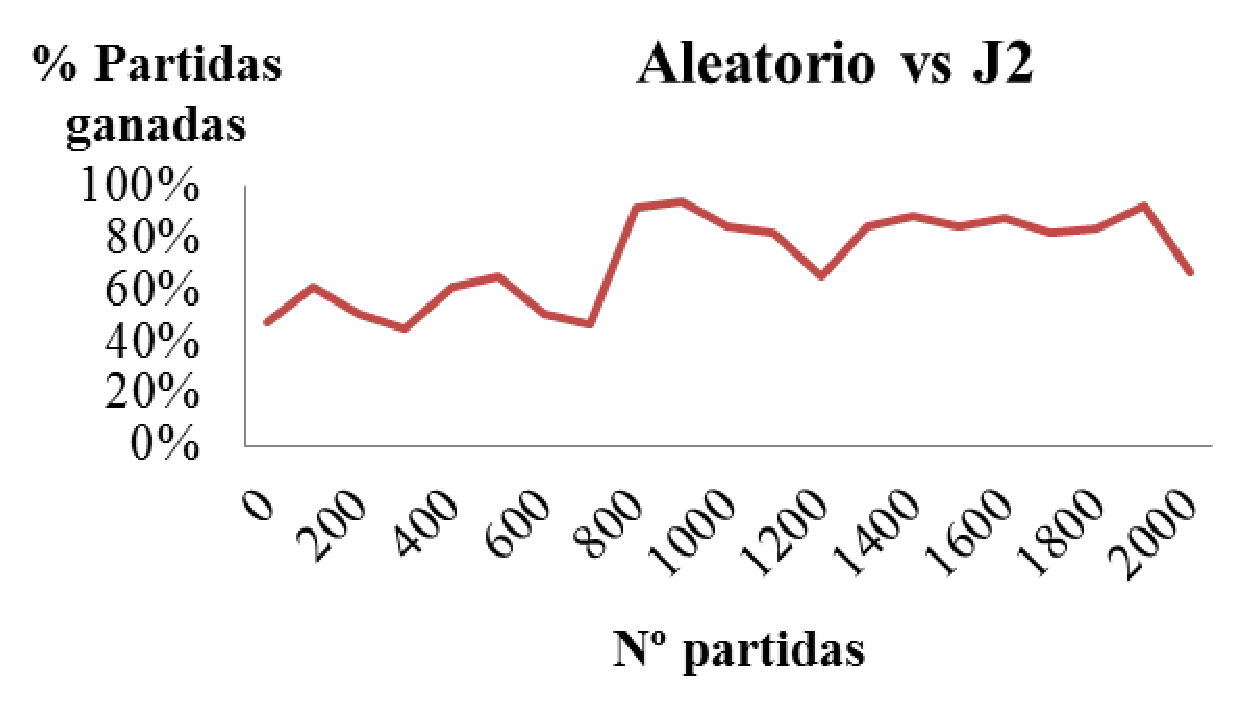
\includegraphics[scale=0.3]{contenido/cap7/imagenes/entrenamientoSecuencia2.eps}
		\caption[Secuencia de entrenamiento 2]{Secuencia 2.}
		\label{fig:secuencia2}
	\end{minipage}
\end{figure}

\begin{figure}[t]
	\centering
	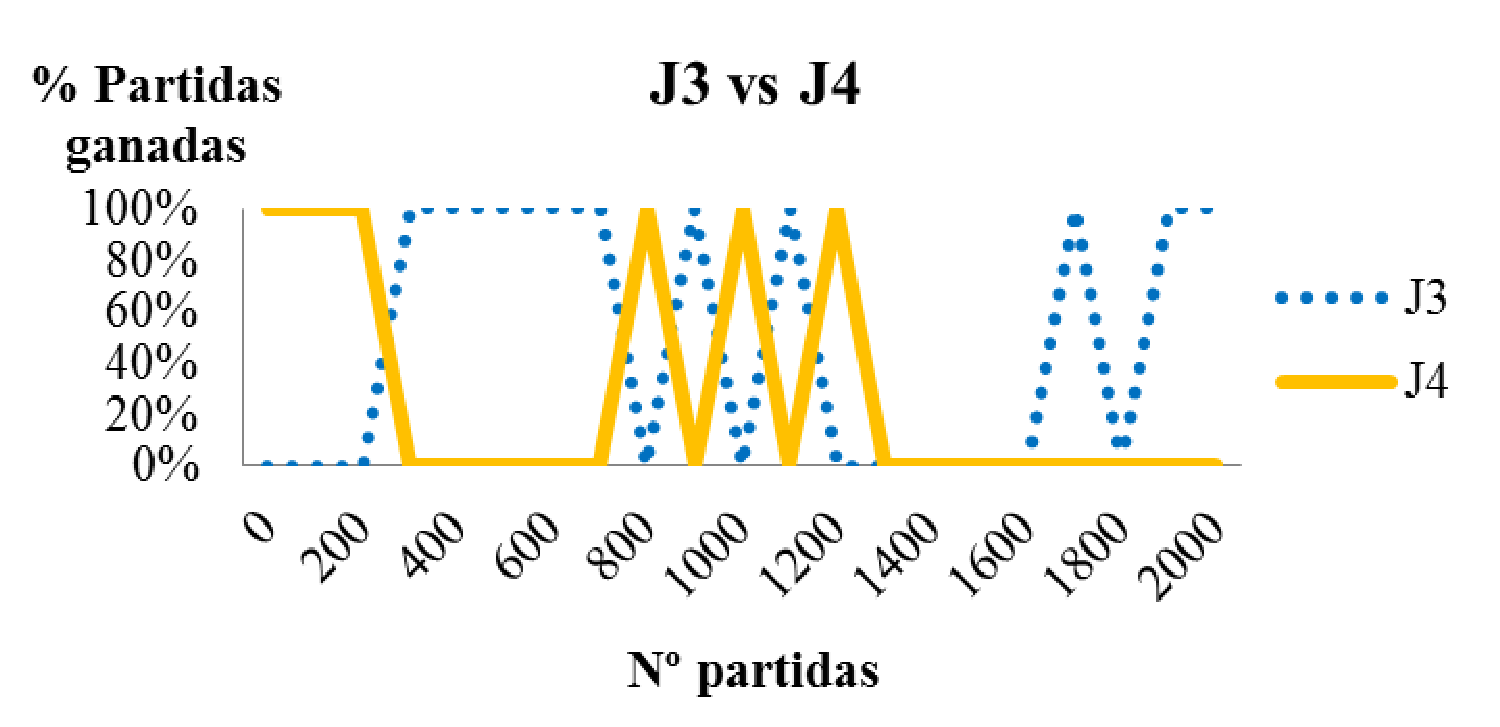
\includegraphics[scale=0.3]{contenido/cap7/imagenes/entrenamientoSecuencia3.eps}
	\caption[Secuencia de entrenamiento 3]{Secuencia 3.}
	\label{fig:secuencia3}
\end{figure} 

Con los jugadores entrenados, cada uno jugará 100 partidas frente a una estrategia aleatoria para comparar los resultados de los entrenamientos.
La tabla~\ref{tab:comparativa_resultados_entrenamientos} y la figura~\ref{fig:comparativa_resultados_entrenamientos} presentan los resultados de estas pruebas.
Se observa que en el caso del jugador J4 se han obtenido mejores resultados que para el jugador J2.
Recordemos que J4 entrena frente a otro jugador que aprende simultáneamente (J3), mientras J2 entrena frente a un jugador aleatorio.

\begin{table}[t]
\centering
\caption{Resultados frente a una estrategia aleatoria.}
\label{tab:comparativa_resultados_entrenamientos}
\begin{tabular}{lcccc}
\hline
\textbf{Jugador 1:} & \textbf{J1} & \textbf{Aleatorio} & \textbf{J3} & \textbf{Aleatorio} \\
\textbf{Jugador 2:} & \textbf{Aleatorio} & \textbf{J2} & \textbf{Aleatorio} & \textbf{J4} \\
%\hline
\textbf{Gana jugador 1} & 99\% & 33\% & 78\% & 7\% \\
\textbf{Empate} & 0\% & 2\% & 3\% & 1\% \\
\textbf{Gana jugador 2}  & 1\% & 65\% & 19\% & 92\% \\
\hline
\end{tabular}
\end{table} 

\begin{figure}[t]
	\centering
	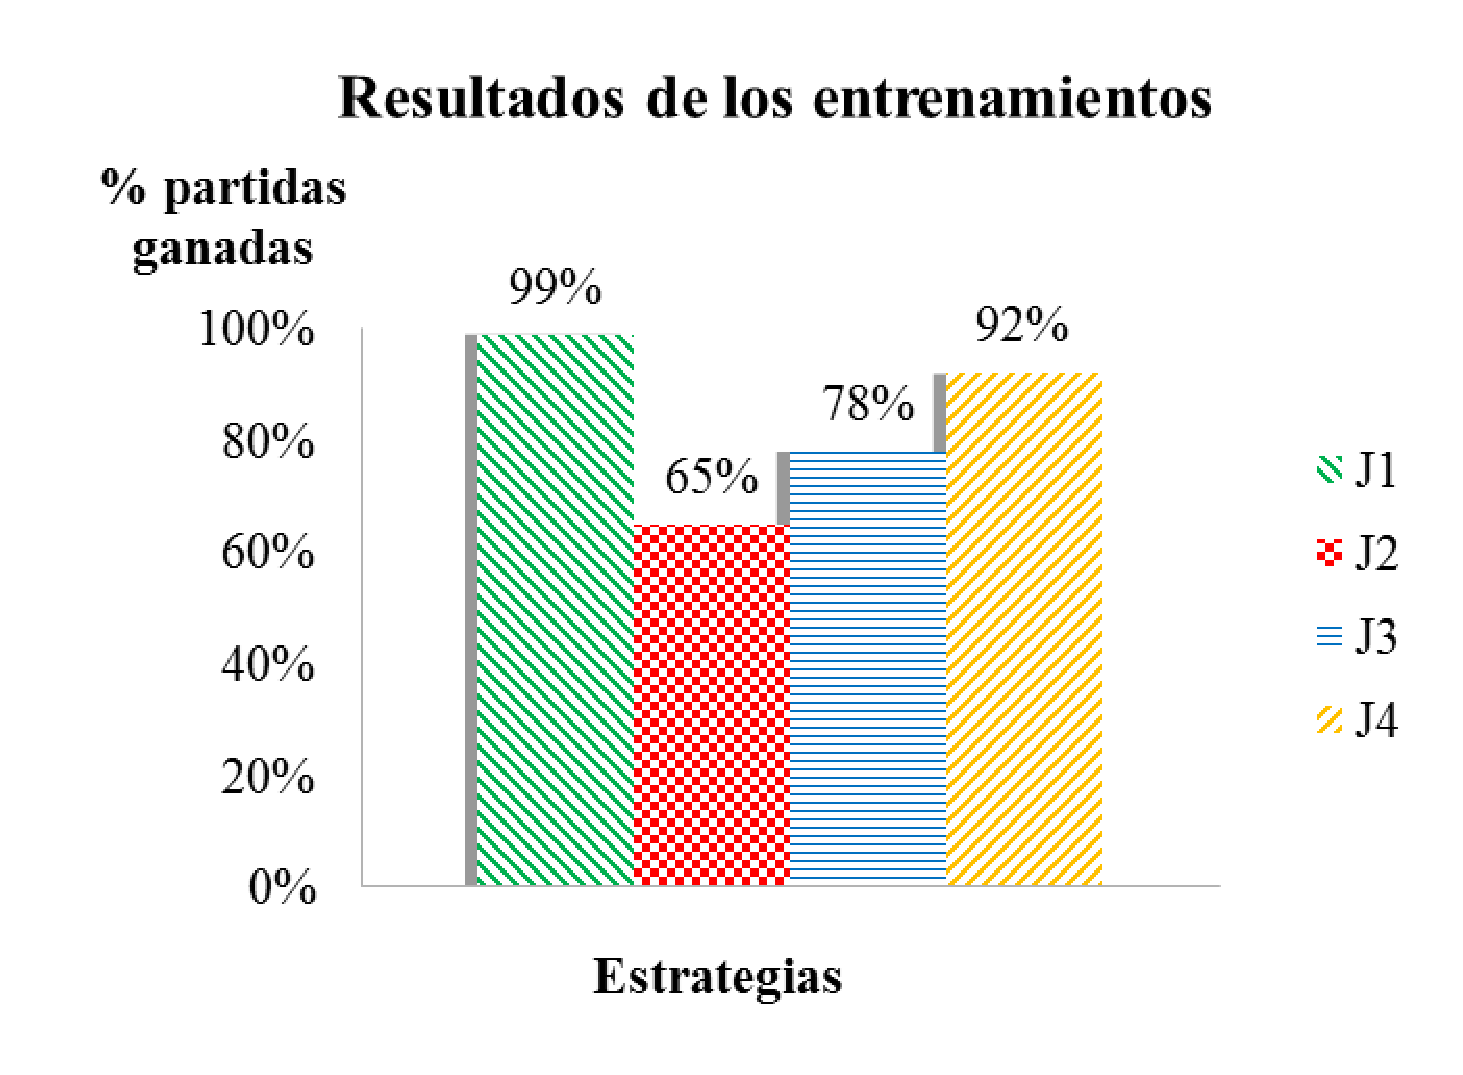
\includegraphics[scale=0.3]{contenido/cap7/imagenes/entrenamientosResultados.eps}
	\caption{Resultados de los entrenamientos.}
	\label{fig:comparativa_resultados_entrenamientos}
\end{figure} 

%\clearpage	% le dice a Latex que suelte todas las figuras en una página y comience una página nueva (detallado en los apuntes de los indios).

\section{Comparativa de estrategias}  
\label{sec:comparativa_estrategias}
En este sección se comparan algunas de las estrategias desarrolladas; para ello se analizan varios estados de los juegos y se realizan algunas simulaciones.

En primer lugar se compara la estrategia minimax frente a su versión mejorada con poda alfa-beta.
También se comparan las dos versiones desarrolladas del método de Monte-Carlo.
En estos casos se usará el juego del Conecta-4.
Por último se realizan varias pruebas en forma de simulaciones, donde cada estrategia juega frente a un jugador aleatorio en el juego del Go.

\subsection{Minimax y Alfa-Beta}
\label{ssec:comparativa_minimaxVSalfabeta}
A continuación se compara la eficacia de un jugador con poda alfa-beta frente a un jugador con el algoritmo minimax en su versión simple.
Se estudian dos estados del juego del Conecta-4 en un tablero 6x7: un estado inicial del juego y un estado intermedio en el que ya se han realizado varios movimientos.

\bigskip
Dado el estado inicial del juego del Conecta-4 (figura~\ref{fig:comparativa_minimax_alfabeta1}) se realiza una búsqueda en el árbol de juegos mediante las estrategias minimax y alfa-beta para obtener el mejor movimiento.
En ambos casos se limita la profundidad máxima de búsqueda al nivel 7.

\begin{figure}[b]
	\centering
	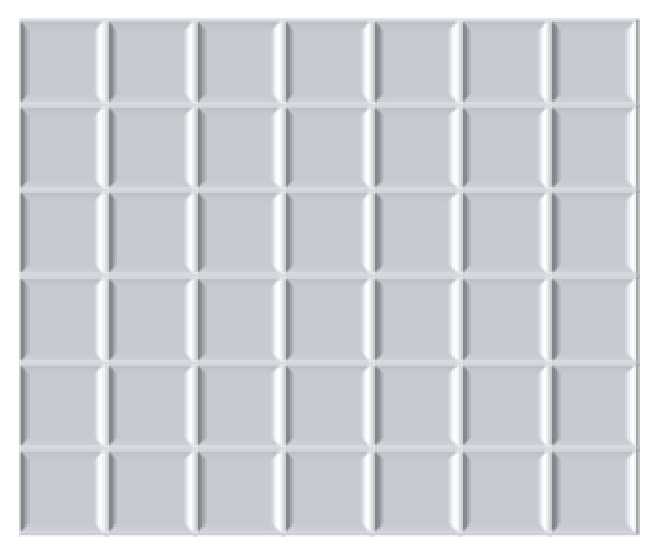
\includegraphics[scale=0.4]{contenido/cap7/imagenes/ckEstadoInicial.eps}
	\caption{Estado inicial del Conecta-4.}
	\label{fig:comparativa_minimax_alfabeta1}
\end{figure} 

En la tabla~\ref{tab:comparativa_minimax_alfabeta1} se muestran las estadísticas sobre la búsqueda del mejor movimiento posible.
Para cada nivel (desde 0 hasta la profundidad máxima) se muestra el número de nodos examinados en ese nivel por cada estrategia.
También se muestra el tiempo empleado en realizar la búsqueda.

\begin{table}[b]
\centering
\caption{Estadísticas de las estrategias minimax y alfa-beta.}
\label{tab:comparativa_minimax_alfabeta1}
\begin{tabular}{c|l|l}
\hline
& \multicolumn{1}{c|}{\textbf{Minimax}} & \multicolumn{1}{c}{\textbf{Alfa-Beta}}\\
\textbf{Profundidad} & \textbf{Nº nodos examinados} & \textbf{Nº nodos examinados} \\
%\hline
0 & 1 & 1 \\
1 & 7 & 7 \\
2 & 49 & 27 \\ 
3 & 343 & 118 \\
4 & 2.401 & 427 \\
5 & 16.807 & 1.621 \\
6 & 117.649 & 5.908 \\
7 & 823.536 & 22.103 \\
\hline
\textbf{Total:} & 960.793 nodos & 30.212 nodos \\
\textbf{Tiempo:} & 12,32 segundos & 1,10 segundos \\
\hline
\end{tabular}
\end{table} 

El mejor movimiento devuelto por ambas estrategias se muestra en la figura~\ref{fig:comparativa_minimax_alfabeta1Movimiento}, que corresponde a soltar una ficha en la columna central; obviamente tanto minimax como alfa-beta devuelven el mismo movimiento.
Se observa el importante ahorro de tiempo usando la poda alfa-beta; en algunos casos se llegan a podar ramas completas del árbol de juegos.

\begin{figure}[t]
	\centering
	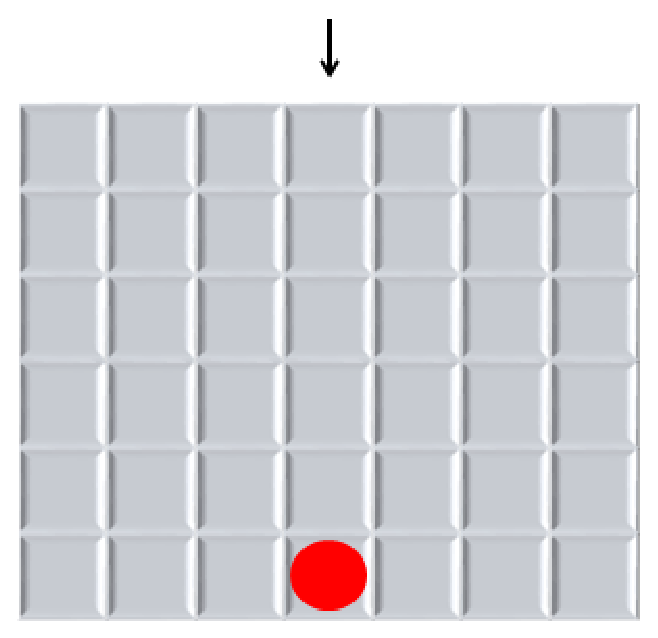
\includegraphics[scale=0.4]{contenido/cap7/imagenes/ckEstadoInicialMovimiento.eps}
	\caption[Mejor movimiento de minimax y alfa-beta en el Conecta-4 (I)]{Mejor movimiento devuelto por las estrategias minimax y alfa-beta para el estado inicial del Conecta-4.}
	\label{fig:comparativa_minimax_alfabeta1Movimiento}
\end{figure} 

\bigskip
En el siguiente ejemplo se considera un tablero ya inicializado correspondiente al estado mostrado en la figura~\ref{fig:comparativa_minimax_alfabeta2}. 
Le toca mover al primer jugador (\textit{MAX}) que juega con \textit{O}.
En este caso las estrategias minimax y alfa-beta disponen de un límite de tiempo de un segundo para realizar la búsqueda del mejor movimiento.

\begin{figure}[!h]
	\centering
	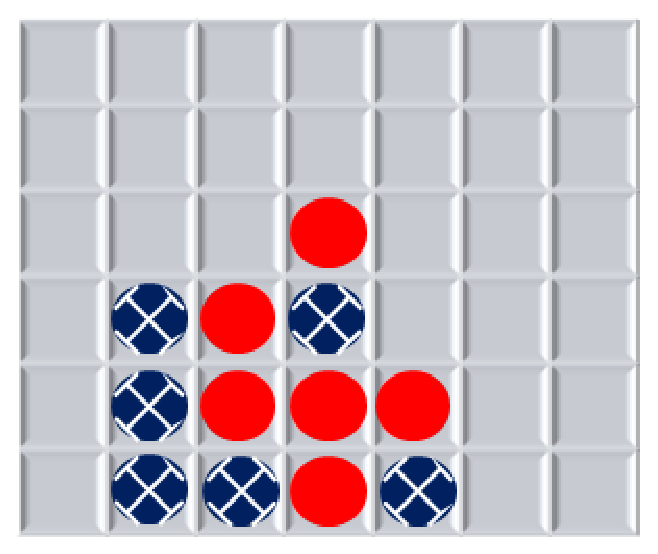
\includegraphics[scale=0.4]{contenido/cap7/imagenes/ckEstadoActual.eps}
	\caption{Estado inicializado del Conecta-4.}
	\label{fig:comparativa_minimax_alfabeta2}
\end{figure} 

La tabla~\ref{tab:comparativa_minimax_alfabeta2} presenta las estadísticas obtenidas en esta prueba.
Se muestra el número de nodos expandidos en cada iteración, teniendo en cuenta que las estrategias realizan una profundización progresiva.

\begin{table}[!h]
\centering
\caption[Estadísticas de minimax y alfa-beta con límite de tiempo]{Estadísticas de las estrategias minimax y alfa-beta con límite de tiempo.}
\label{tab:comparativa_minimax_alfabeta2}
\begin{tabular}{c|l|l}
\hline
& \multicolumn{1}{c|}{\textbf{Minimax}} & \multicolumn{1}{c}{\textbf{Alfa-Beta}}\\
\textbf{Iteración} & \textbf{Nº nodos expandidos} & \textbf{Nº nodos expandidos} \\
%\hline
0 & 1 & 1 \\
1 & 8 & 8 \\
2 & 57 & 37 \\ 
3 & 357 & 131 \\
4 & 2326 & 607 \\
5 & 14492 & 1721 \\
6 & 66420 & 2184 \\
7 &  & 13909 \\
8 &  & 57439 \\
\hline
\textbf{Total:} & 83661 nodos & 76037 nodos\\
\hline
\end{tabular}
\end{table} 

Mientras que minimax alcanza una profundidad máxima de búsqueda de 6 niveles, alfa-beta consigue llegar hasta una profundidad de 8 niveles en el mismo tiempo.
El número de nodos expandidos con la estrategia alfa-beta es sólo orientativo pues en cada profundización pueden expandirse más o menos nodos dependiendo de si se producen o no podas.


La figura~\ref{fig:comparativa_minimax_alfabeta2Movimiento} muestra el mejor movimiento devuelto por las dos estrategias, que en este caso es también el mismo, aunque ya no tienen por qué coincidir, pues cada estrategia evalúa los estados a diferente profundidad.
El estado dado era favorable para el segundo jugador (\textit{MIN}), de ahí que el mejor movimiento posible para \textit{MAX} sea obligado en la segunda columna para no perder la partida.
\textit{MIN} juega una partida perfecta y ganaría en la siguiente jugada si \textit{MAX} no moviera en la primera columna.

\begin{figure}[!h]
	\centering
	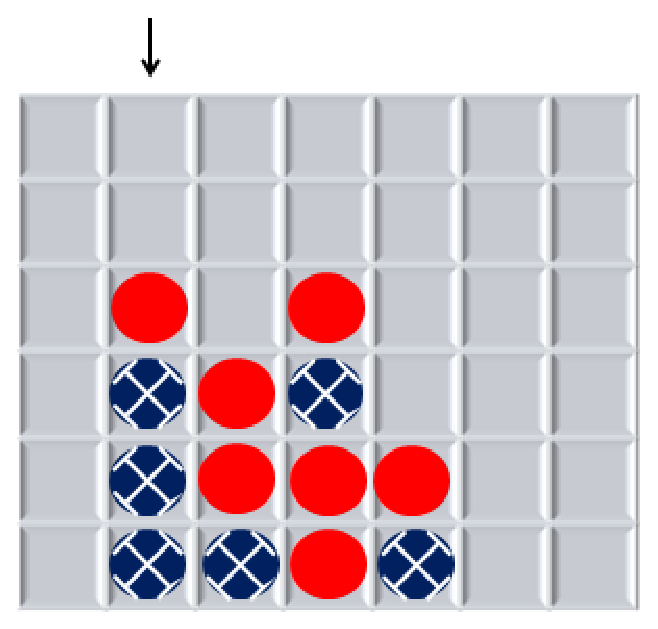
\includegraphics[scale=0.4]{contenido/cap7/imagenes/ckEstadoActualMovimiento.eps}
	\caption[Mejor movimiento de minimax y alfa-beta en el Conecta-4 (II)]{Mejor movimiento de minimax y alfa-beta para el estado de la figura~\ref{fig:comparativa_minimax_alfabeta2}.}
	\label{fig:comparativa_minimax_alfabeta2Movimiento}
\end{figure} 

\subsection{Monte-Carlo y Monte-Carlo Tree Search}
\label{ssec:comparativa_mcVSmctreesearch}
Este apartado compara las dos estrategias que usan el método de Monte-Carlo.
Para ello se estudian los resultados de enfrentar ambas estrategias en función del límite de tiempo disponible para decidir el mejor movimiento.

Se considera el juego del Conecta-4 en un tablero 6x7.
Cada prueba consiste en 100 partidas con un límite de tiempo para cada jugador a la hora de decidir los movimientos.
Para cada prueba se incrementa el límite de tiempo en un segundo, salvo para la última prueba que tiene un límite de 15 segundos.\footnote{Cada una de las pruebas puede durar varias horas, de ahí que se haya escogido el juego del Conecta-4 en lugar del juego del Go para realizar este experimento; incluso en el juego del Conecta-4 en un tablero 6x7 la duración media de cada prueba ha sido de 4 horas.}

En el primer caso, el jugador que mueve en primer lugar usa el método de Monte-Carlo básico y el segundo jugador el método Monte-Carlo Tree Search.
La tabla~\ref{tab:comparativa_montecarlo1} muestra los resultados de las pruebas realizadas.
La figura~\ref{fig:comparativa_montecarlo1} muestra estos datos de forma gráfica.

En el siguiente caso, el primer jugador usa el método Monte-Carlo Tree Search y el segundo jugador el método básico de Monte-Carlo.
Los resultados de esta pruebas se muestran en la tabla~\ref{tab:comparativa_montecarlo2} y en la figura~\ref{fig:comparativa_montecarlo2}.

En ambos casos, jugando como primer jugador o como segundo jugador, se observa claramente que el método Monte-Carlo Tree Search obtiene mejores resultados que el método Monte-Carlo basado simplemente en las simulaciones.

\begin{table}[!h]
\centering
\caption[Comparativa de los métodos de Monte-Carlo (I)]{Comparativa del método Monte-Carlo frente a Monte-Carlo Tree Search.}
\label{tab:comparativa_montecarlo1}
\begin{tabular}{cccc}
\hline
\textbf{Límite de tiempo (s)} & \textbf{Gana jug.1 (MC)} & \textbf{Empate} & \textbf{Gana jug.2 (MC Tree Search)}\\
%\hline
1 & 16\% &	5\% &	79\% \\
2 & 12\% &	1\% &	87\% \\
3 & 11\% &	1\% &	88\% \\
4 & 3\% &	0\% &	97\%  \\
5 & 3\% &	1\% &	96\%  \\
6 & 4\% &	2\% &	94\%  \\
7 & 4\% &	0\% &	96\%  \\
8 & 3\% &	1\% &	96\% \\
9 & 3\% &	1\% &	96\%  \\
10 & 3\% &	3\% &	94\% \\
15 & 1\% &	0\% &	99\% \\
\hline
\end{tabular}
\end{table} 

\begin{figure}[!h]
	\centering
	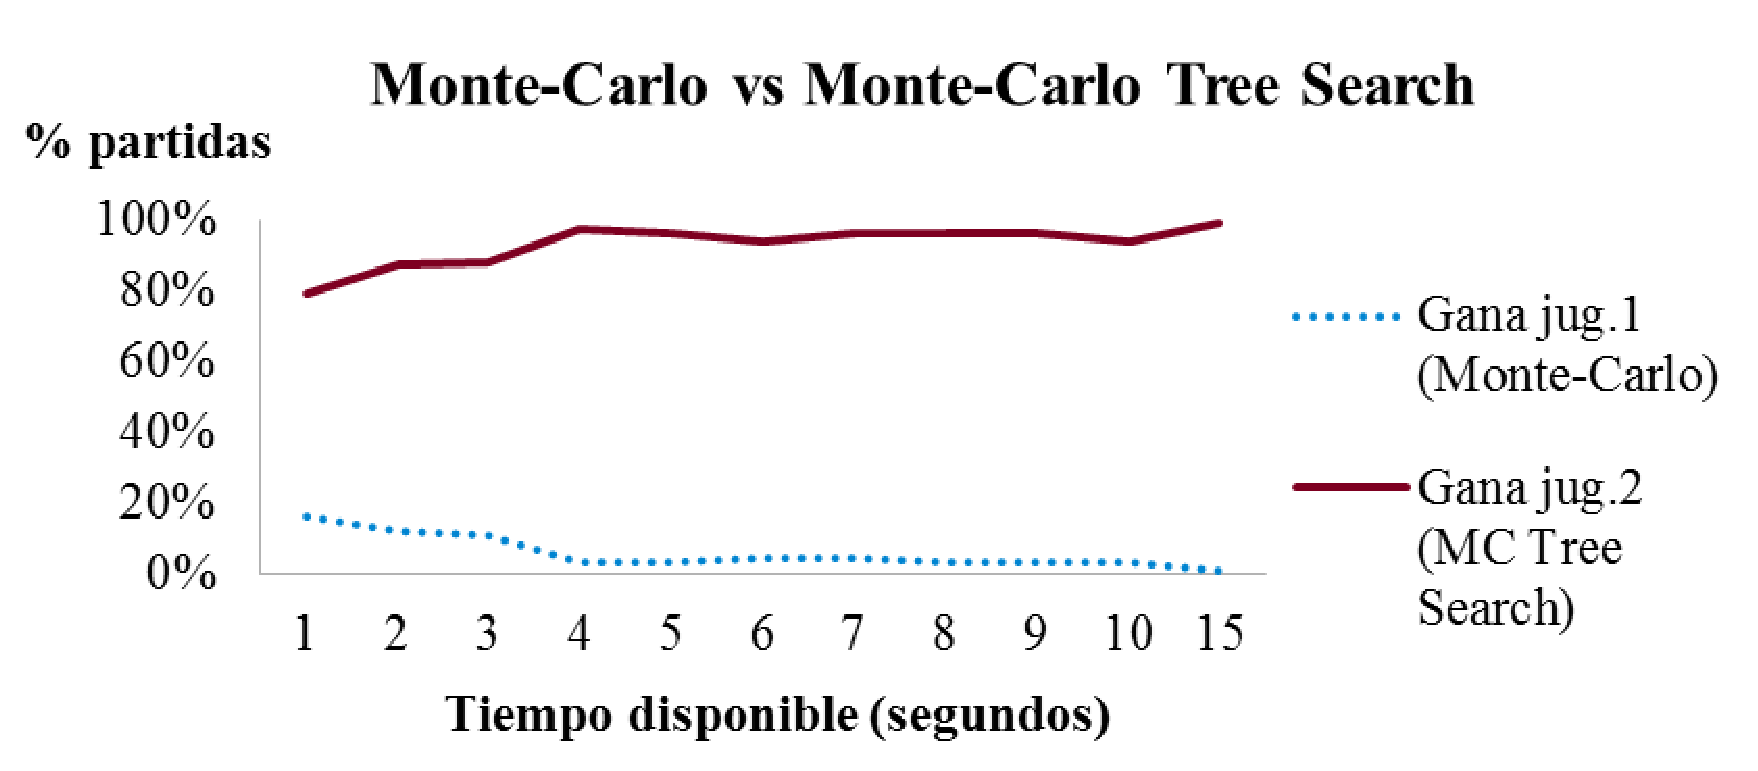
\includegraphics[scale=0.4]{contenido/cap7/imagenes/montecarlo1.eps}
	\caption[Comparativa de los métodos de Monte-Carlo (I)]{Gráfica comparativa de los métodos de Monte-Carlo (datos de la tabla~\ref{tab:comparativa_montecarlo1}).}
	\label{fig:comparativa_montecarlo1}
\end{figure} 

\begin{table}[!h]
\centering
\caption[Comparativa de los métodos de Monte-Carlo (II)]{Comparativa del método Monte-Carlo Tree Search frente a Monte-Carlo.}
\label{tab:comparativa_montecarlo2}
\begin{tabular}{cccc}
\hline
\textbf{Límite de tiempo (s)} & \textbf{Gana jug.1 (MC Tree Search)} & \textbf{Empate} & \textbf{Gana jug.2 (MC)}\\
%\hline
1 & 79\% &	3\% &	18\% \\
2 & 83\% &	6\% &	11\% \\
3 & 90\% &	7\% &	3\% \\
4 & 87\% &	6\% &	7\% \\
5 & 96\% &	4\% &	0\% \\
6 & 94\% &	4\% &	2\% \\
7 & 95\% &	2\% &	3\% \\
8 & 95\% &	3\% &	2\% \\
9 & 98\% &	2\% &	0\% \\
10 & 98\% &	1\% &	1\% \\
15 & 99\%	& 1\%	 & 0\% \\
\hline
\end{tabular}
\end{table} 

\begin{figure}[!h]
	\centering
	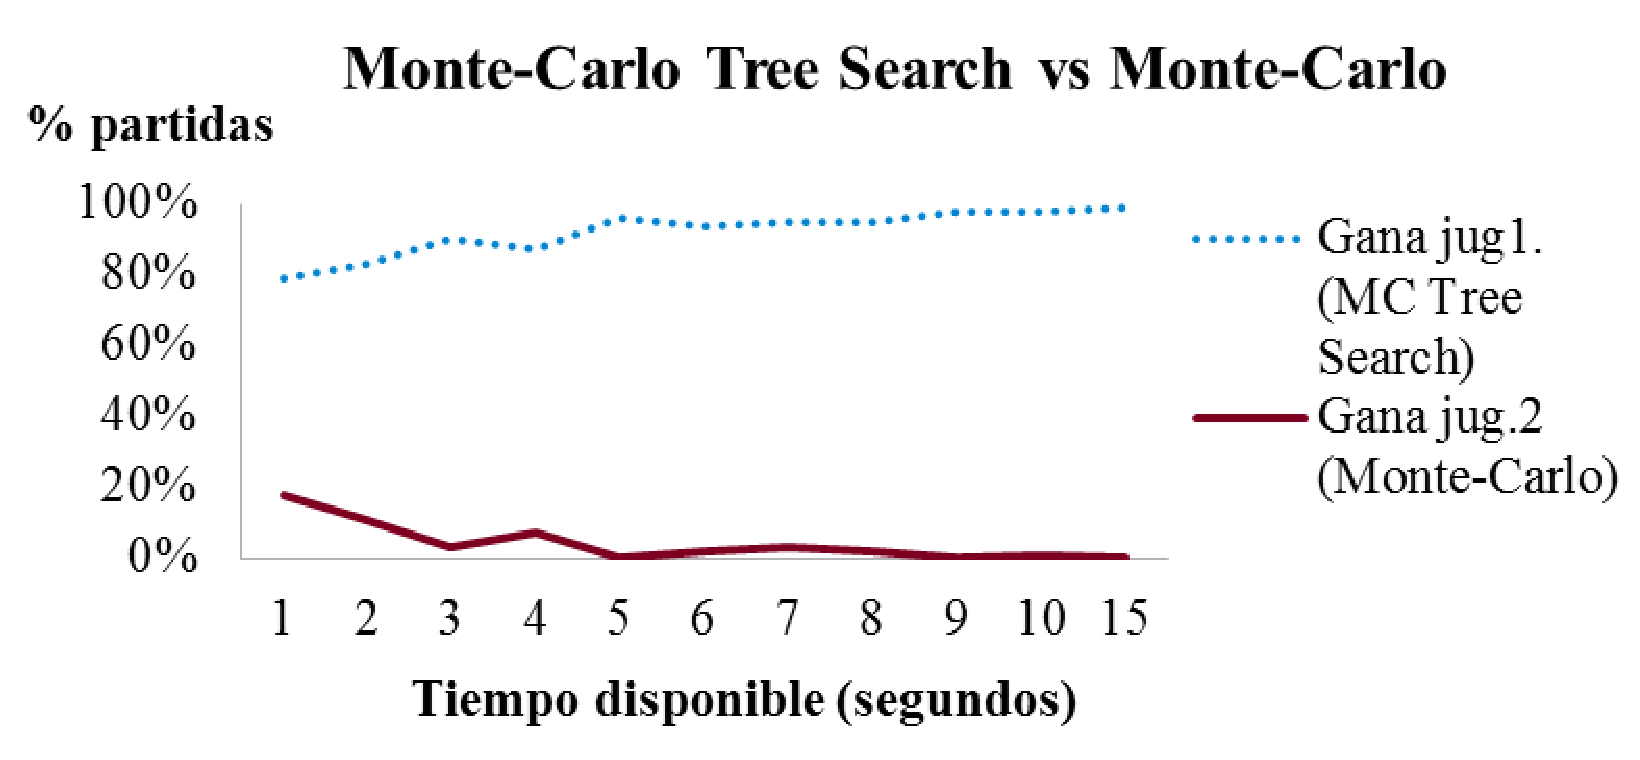
\includegraphics[scale=0.4]{contenido/cap7/imagenes/montecarlo2.eps}
	\caption[Comparativa de los métodos de Monte-Carlo (I)]{Gráfica comparativa de los métodos de Monte-Carlo (datos de la tabla~\ref{tab:comparativa_montecarlo2}).}
	\label{fig:comparativa_montecarlo2}
\end{figure} 


\subsection{Comparativa de estrategias en el Go}
\label{ssec:comparativa_estrategias_go}
A continuación se realiza una comparativa de varias estrategias en el juego del Go.

Se considera un tablero 9x9 inicialmente vacío, con las reglas de puntuación japonesas y sin puntos de ventaja para el segundo jugador.
Las estrategias a comparar son un jugador aleatorio, un jugador evaluador heurístico (\texttt{JugadorEvaluar}), un jugador minimax, un jugador con poda alfa-beta, un jugador Monte-Carlo y otro Monte-Carlo Tree Search.
El heurístico empleado tanto para el jugador evaluador heurístico como para minimax y alfa-beta ha sido el evaluador basado en la puntuación según las reglas japonesas.
Todas las estrategias (salvo el \texttt{JugadorEvaluar}) disponen de un segundo para encontrar el mejor movimiento.

La tabla~\ref{tab:comparativa_estrategias1} presenta los resultados de las pruebas para el caso en el que las estrategias juegan como primer jugador.
Cada estrategia ha jugado 100 partidas frente a un jugador aleatorio.
La figura~\ref{fig:comparativa_estrategias1} muestra de forma gráfica los resultados obtenidos.

Los resultados de las estrategias cuando son usadas por el segundo jugador se muestran en la tabla~\ref{tab:comparativa_estrategias2}.
La figura~\ref{fig:comparativa_estrategias2} muestra de forma gráfica estos resultados.
En este caso también se han jugado 100 partidas con cada estrategia frente a un jugador aleatorio.

\begin{table}[t]
\centering
\caption[Comparativa de estrategias en el Go (I)]{Comparativa de las estrategias usadas por el primer jugador en el Go.}
\label{tab:comparativa_estrategias1}
\begin{tabular}{lcccccc}
\hline
\textbf{Jugador 1:} & \textbf{Aleatorio} & \textbf{Ev. Heur.} & \textbf{Minimax} & \textbf{Alfa-Beta} & \textbf{MC} & \textbf{MC Tree Search} \\
%\hline
\textbf{Gana} & 47\% & 98\% & 89\% & 96\% & 83\% & 88\% \\
\textbf{Empata} & 4\% & 1\% & 0\% & 0\% & 1\% & 2\% \\
\textbf{Pierde} & 49\% & 1\% & 11\% & 4\% & 16\% & 10\% \\
\hline
\end{tabular}
\end{table} 

\begin{figure}[!h]
	\centering
	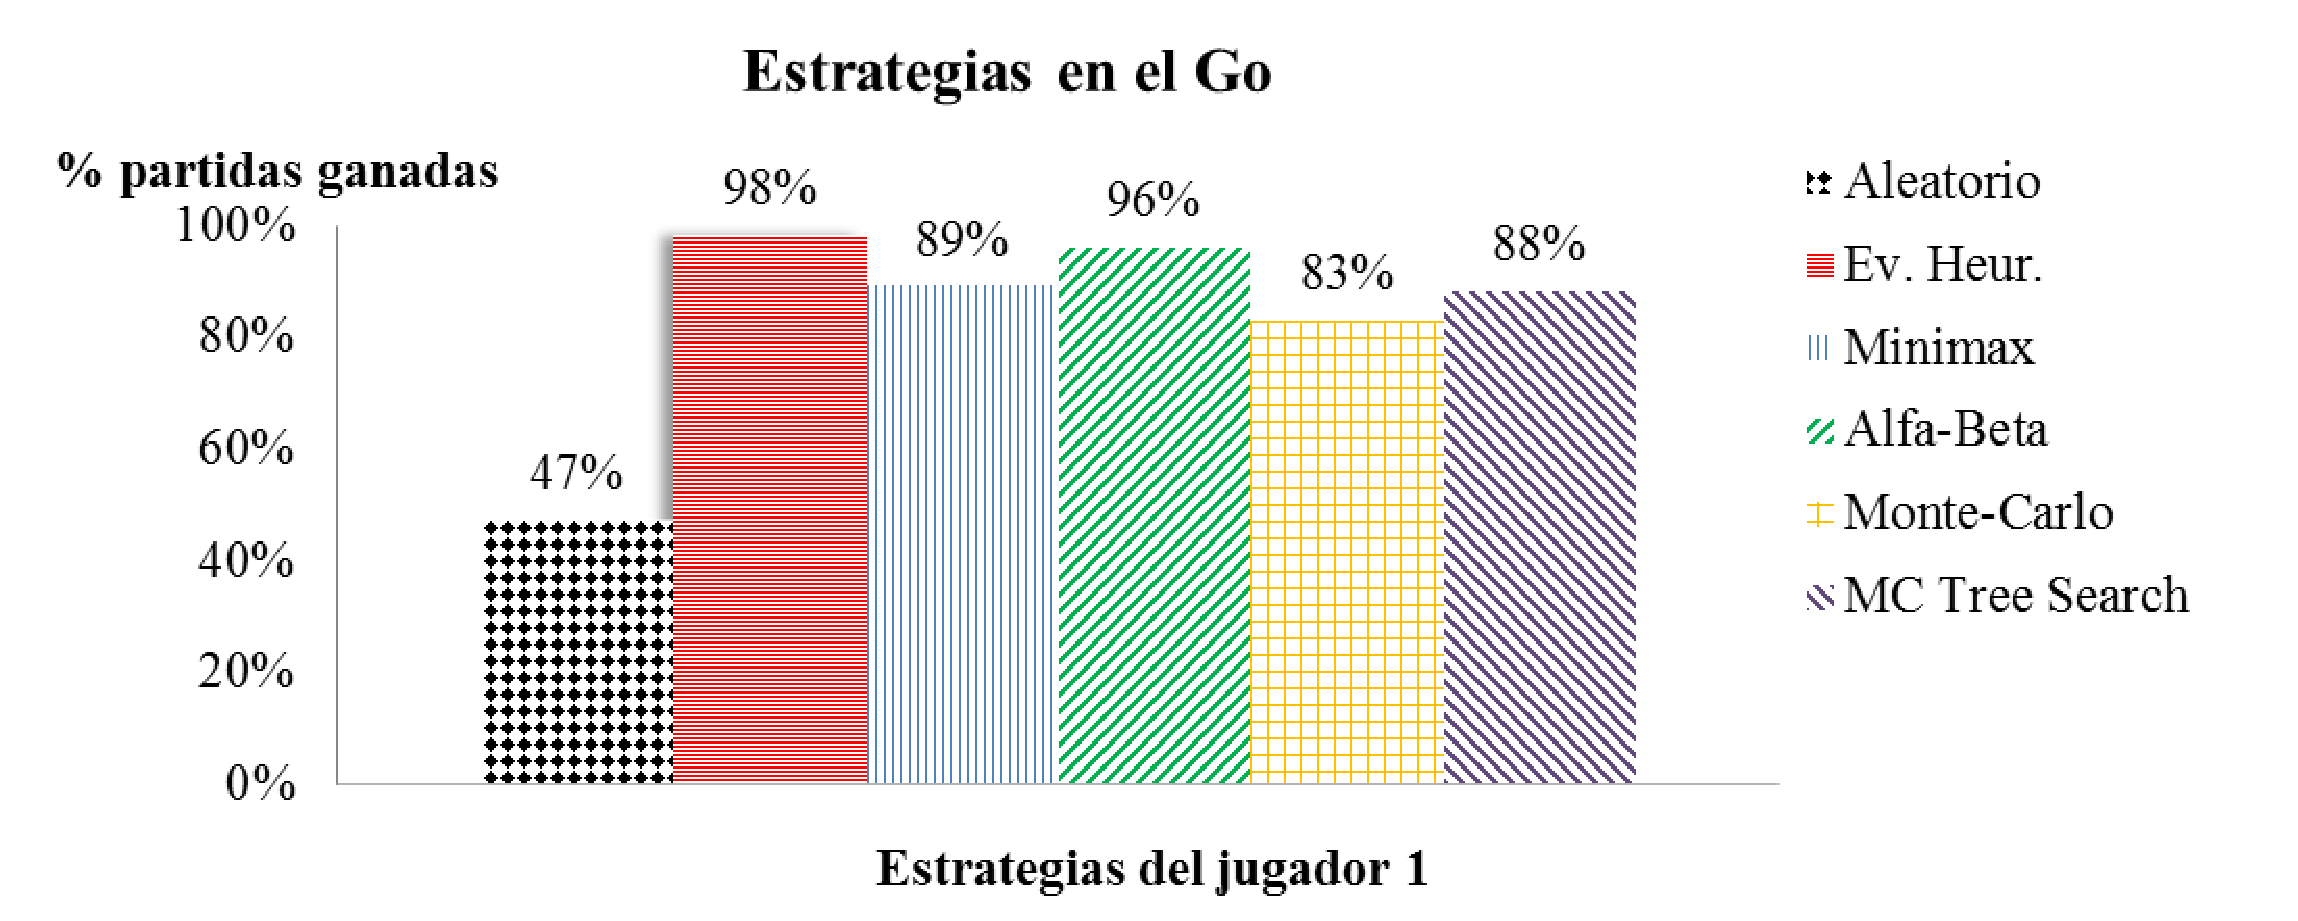
\includegraphics[scale=0.3]{contenido/cap7/imagenes/estrategiasGo1.eps}
	\caption[Comparativa de estrategias en el Go (I)]{Gráfica comparativa de las estrategias del primer jugador en el juego del Go.}
	\label{fig:comparativa_estrategias1}
\end{figure} 

\begin{table}[t]
\centering
\caption[Comparativa de estrategias en el Go (II)]{Comparativa de las estrategias usadas por el segundo jugador en el Go.}
\label{tab:comparativa_estrategias2}
\begin{tabular}{lcccccc}
\hline
\textbf{Jugador 2:} & \textbf{Aleatorio} & \textbf{Ev. Heur.} & \textbf{Minimax} & \textbf{Alfa-Beta} & \textbf{MC} & \textbf{MC Tree Search} \\
%\hline
\textbf{Gana} & 49\% & 94\% & 87\%  & 89\% & 80\% & 64\% \\
\textbf{Empata} & 4\% & 0\% & 1\% & 0\% & 0\% & 2\% \\
\textbf{Pierde} & 47\% & 6\%  & 12\% & 11\% & 20\% & 34\% \\
\hline
\end{tabular}
\end{table} 

\begin{figure}[!h]
	\centering
	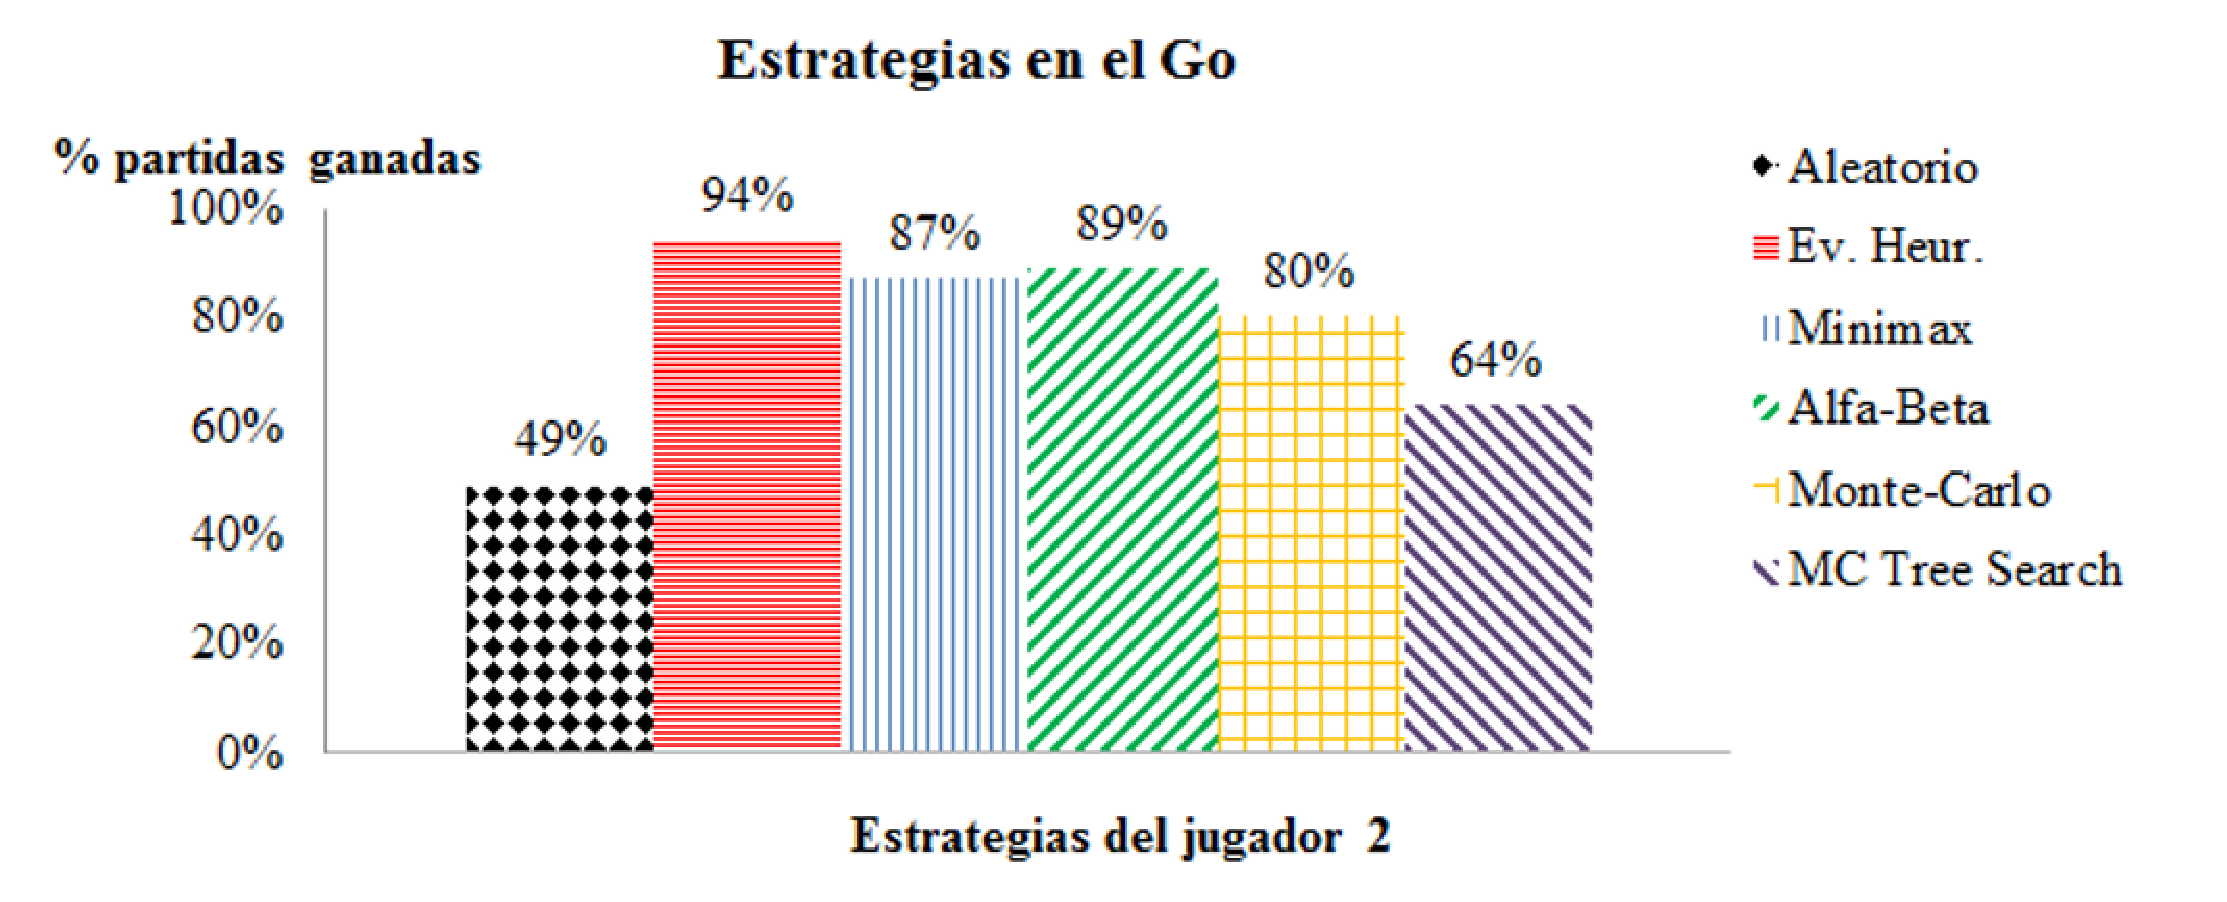
\includegraphics[scale=0.3]{contenido/cap7/imagenes/estrategiasGo2.eps}
	\caption[Comparativa de estrategias en el Go (II)]{Gráfica comparativa de las estrategias del segundo jugador en el juego del Go.}
	\label{fig:comparativa_estrategias2}
\end{figure} 

El evaluador heurístico (\texttt{JugadorEvaluar}) obtiene mejores resultados que minimax y alfa-beta porque examina completamente el primer nivel del árbol de estados.
Minimax y alfa-Beta realizan la búsqueda del mejor movimiento primero en profundidad y en un sólo segundo no les da tiempo a examinar el primer nivel completo.

El método de Monte-Carlo básico obtiene mejores resultados en este caso que Monte-Carlo Tree Search.
Esto se debe a que las simulaciones de Monte-Carlo Tree Search tardan más en ejecutarse que las simulaciones simples de Monte-Carlo.
Un único segundo es muy poco tiempo para realizar las simulaciones de Monte-Carlo Tree Search en un juego como el Go, ya que tanto el árbol de búsqueda como el árbol que se genera son enormes.
Aumentando el tiempo disponible se mejora esta estrategia igual que ocurría en el experimento de la sección~\ref{ssec:comparativa_mcVSmctreesearch}.
